The main resource used in this work is Crazyflie, an open platform produced by Bitcraze~\cite{bitcraze} 
that offers an ecosystem of products and open-source libraries that allow people to develop new functionality for aerial drones. 

The nano-drone Crazyflie 2.1 of the platform is perfect for facilitating human-drone interactions.
With their small size, it is simpler and safer to conduct HDI experiments. 

The key feature of this platform is that it offers a set of expansion decks that can extend the capabilities of the drone with new sensors. 
Expansion decks can be mounted on the drones very easily, and they are immediately ready to be used to compose the desired configuration in the application of interest.

In the field of HDI, it is essential to be ready to rapidly change for adapting to new situation.
Given its modularity and high versatility, this platform perfectly fits as a baseline for developing an easy, high-level environment for programming drones.

The aim of this chapter is to present an overview of the Crazyflie platform to provide basic knowledge of its tools and surrounding environment.

\section{Ecosystem Overview}\label{sec:ecosystem_oveerview}
The Crazyflie platform comprises a set of devices and tools to allow building drone applications. 
It has a modular architecture that makes it possible to build very versatile systems that are adaptable to many situations. 
In Figure~\ref{fig:bitcraze_ecosystem}, we can see an overview of the ecosystem of the entire platform.

The ecosystem of this platform gravitates around its leading actor: the Crazyflie 2.1 nano drone. 
In the basic settings, the drone has minimal sensors and actuators that allow it to fly. 
The platform makes available a set of expansion decks that give the drone additional sensors, making it possible to adapt it to many possible situations.


\sidecaptionvpos{figure}{c}
\begin{SCfigure}[\sidecaptionrelwidth][tb]
    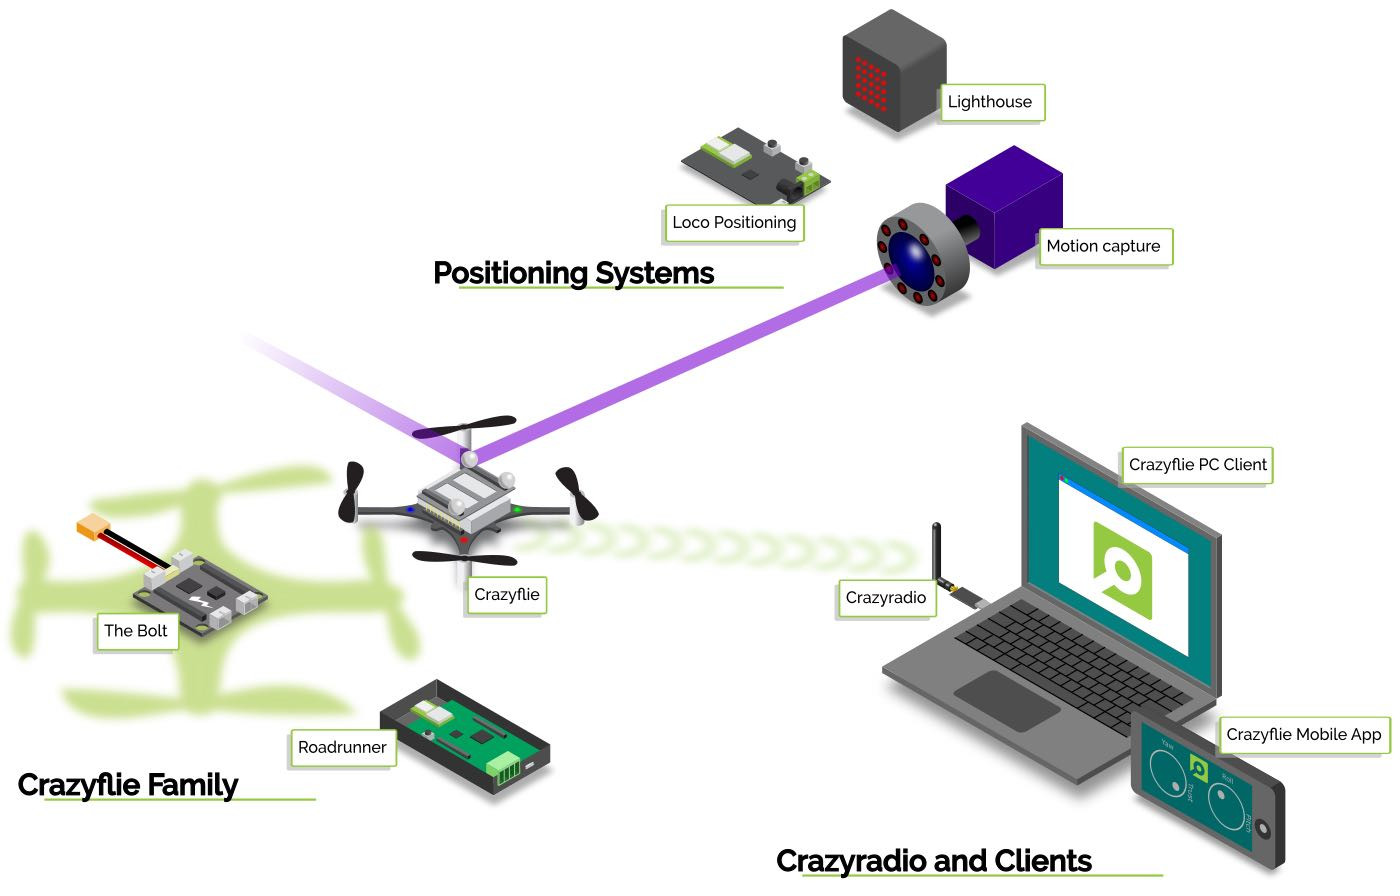
\includegraphics[width=0.5\textwidth]{tools/system_overview}
    \caption[Bitcraze Ecosystem overview]{This picture represents an overview of the Bitcraze Ecosystem~\cite{bitcraze}}
    \label{fig:bitcraze_ecosystem}
\end{SCfigure}


To coordinate the drone's operations, the platform needs a ground station that can be hosted on any computer 
with a Python script interpreter or a mobile phone with a dedicated App installed. 

The communication between the quadcopter and the ground station is handled using a dongle USB (CrazyRadio) or through Bluetooth when using the mobile app.

The platform also offers multiple absolute positioning systems that allow the drone to estimate position in an absolute coordinate system.

\section{Hardware}\label{sec:crazyflie_hardware}
In this section, we will provide an overview of the hardware components of the entire Crazyflie platform. 
We will first analyze the characteristics of the Crazyflie quadcopter used in this work, and then we will briefly introduce the relevant expansion decks. 
We will then give an overview of the hardware components that compose the absolute positioning system adopted for the work: the Lighthouse positioning system.

\subsection{The Drone}\label{subsec:the_quadcopter}
Bitcraze produces a family of drones with similar hardware and firmware but different sizes and properties. 
The target for this work is the principal component of this family, the Crazyflie 2.1, a tiny and versatile quadcopter with a solid and modularized design that falls into the category of nano-drones.

As described in Section~\ref{sec:the_solution}, nano-drones are the most suitable type for conducting investigations around HDI. 
The modular approach owned by Crazyflie 2.1 constitutes another key advantage in the field of HDI; 
the user can easily change the setup to address any possible situation. 

This drone has many hardware components hosted on a single, compact, light base. 
We can identify four main units: computing unit, motor unit, sensor unit, and power unit.

The core of the drone is composed of two Micro Controller Units (MCUs): 
The first is an STM32F4 MCU that handles the main Crazyflie firmware with all the low-level and high-level controls. 
The second MCU, NRF51822, handles the radio communication and power management. 

The motor unit of the Crazyflie 2.1 consists of four brushless DC motors with plastic propellers fixed at the corners of the base with the help of plastic supports.
To control the flight, the drone is equipped with two sensors: a BMI088 sensor, which measures the acceleration along the three coordinates of space plus the angular speed, 
and a BMP388 sensor, which is a high-precision pressure sensor.
The sensor unit of the Crazyflie 2.1, also known as the Inertial Measurement Unit (IMU), is minimal and provides the minimum data that allows the drone to have an almost stable flight.

Its design is robust and simple, easing the assembly and maintenance of its components.
Finally, the power unit is constituted by a 240mAh LiPo battery that allows a flight duration of about 7 minutes. 
The total weight of the drone is 27 grams, and it can lift a payload of 15 grams~\cite{crazyflie}. 


\subsection{Expansion Decks}\label{subsec:expansion_decks}
With only two sensors composing the IMU, the drone has a limited capacity to understand the surrounding environment. 
To overcome this limitation, the drone can be equipped with additional decks that extend its capabilities in sensing, positioning, and visualization.
The platform offers a variety of expansion decks, but for the purpose of our work, only a subset of them has been selected.
Figure~\ref{fig:decks} shows the expansion decks selected, particularly those that can enable in some way the HDI.

\begin{figure}[tb]
    \centering
    \subfloat[Flow deck v2\label{fig:flow_deck}]{
        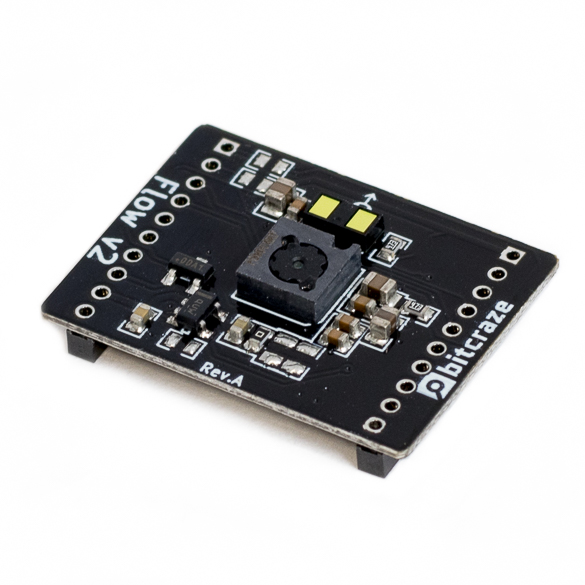
\includegraphics[width=0.16\textwidth]{tools/flow_deck_v2}
    }
    \quad
    \subfloat[Z-ranger deck v2\label{fig:z_ranger_deck}]{
        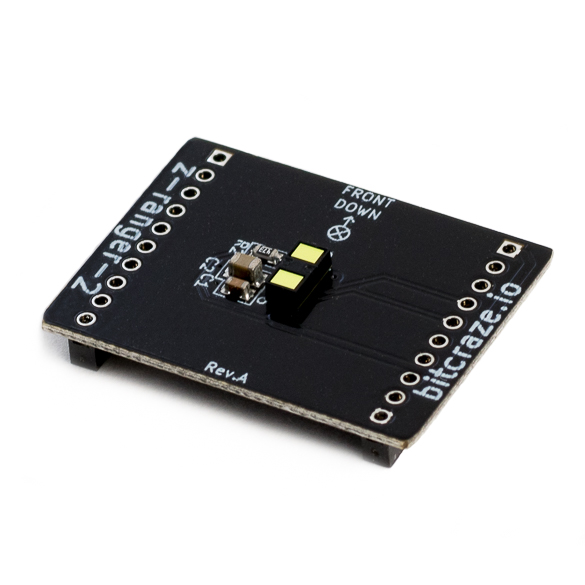
\includegraphics[width=0.16\textwidth]{tools/z-ranger_v2}
    }
    \quad
    \subfloat[Multi-ranger deck\label{fig:multi_ranger_deck}]{
        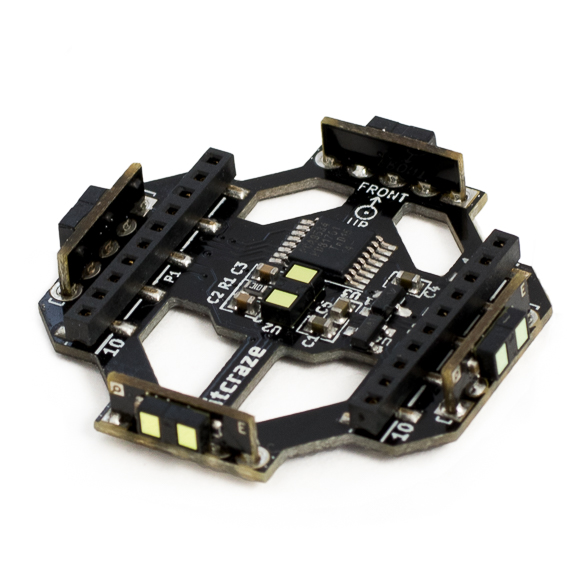
\includegraphics[width=0.16\textwidth]{tools/multi-ranger_deck}
    }
    \quad
    \subfloat[Lighthouse positioning deck\label{fig:lighthouse_deck}]{
        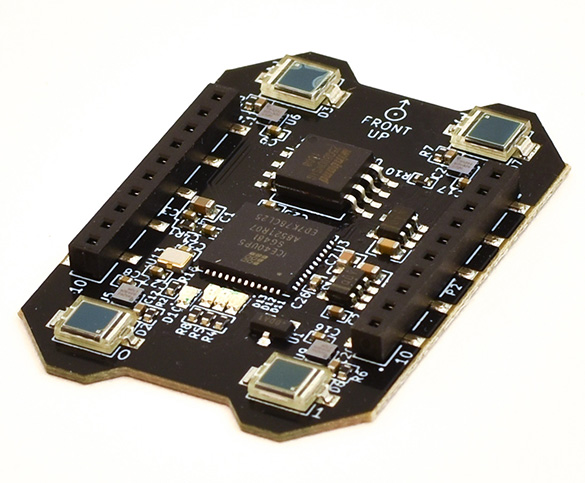
\includegraphics[width=0.16\textwidth]{tools/lighthouse_deck}
    }
    \quad
    \subfloat[AI-deck 1.1\label{fig:ai_deck}]{
        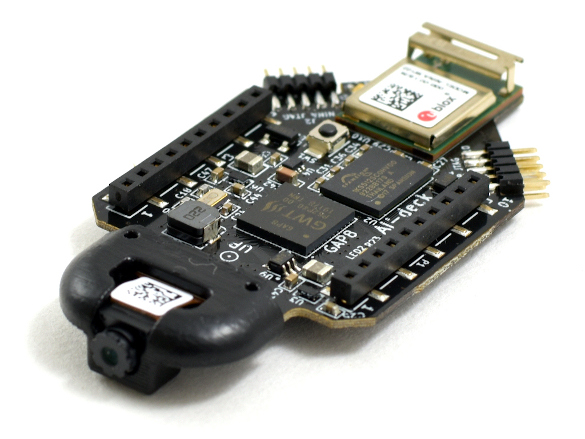
\includegraphics[width=0.16\textwidth]{tools/ai-deck}
    }
    \caption{Expansion decks of Crazyflie 2.1.}\label{fig:decks}
\end{figure}


{\bfseries \scshape Flow deck v2}\label{deck:flow}:\\*
The Flow deck (Figure~\ref{fig:flow_deck}) allows the Crazyflie to understand when it moves in any direction. 
It mounts two sensors: the VL53L1x ToF measures the distance to the ground with high precision up to 4 meters, and the PMW3901 optical flow sensor measures the relative velocity in the x-y plane relative to the ground. 
This expansion deck is a relative positioning system that lets the drone know its position relative to its take-off point.
The precise positioning capabilities provided by the Flow deck can contribute to safer and more intuitive interactions between humans and drones.

{\bfseries \scshape Z-ranger deck v2}\label{deck:z_ranger}:\\*
The Z-ranger deck (Figure~\ref{fig:z_ranger_deck}) is a simplified and cheaper version of the Flow deck v2.
It only measures the distance from the floor up to 4 meters using the same laser sensor VL53L1x ToF.

{\bfseries \scshape Multi-ranger deck}\label{deck:multi_ranger}:\\*
The Multi-ranger deck (Figure~\ref{fig:multi_ranger_deck}) gives the Crazyflie the capability to sense the space around it and react when something is close and for instance, avoid obstacles.
This is done by measuring the distance to objects in the following five directions: front, back, left, right, and up with mm precision up to 4 meters, using five VL53L1x ToF sensors.
With the capability to measure distances in multiple directions, the drone becomes more aware of its surroundings, enabling it to respond dynamically to changes in its environment. 
This deck enables a set of new interactions with humans, allowing them to interact with it directly. 
An example of interaction could be drone navigation using hands; by approaching the hand to one of the sensors, the user can move the drone around.

{\bfseries \scshape Lighthouse positioning deck}\label{deck:lighthouse}:\\*
The Lighthouse deck (Figure~\ref{fig:lighthouse_deck}) is part of the Lighthouse absolute positioning system (See Section~\ref{subsec:lighthouse_hardware}). 
It comprises four TS4231 IR receivers and an ICE40UP5K FPGA to process the signal received.
This expansion deck lets the drone know its position in an absolute coordinate system.
As part of an absolute positioning system, the Lighthouse deck contributes to the precision and accuracy of the drone's spatial awareness. 
This capability can be crucial in applications requiring precise coordination and control during human interactions.
For instance, in choreographed drone performances or collaborative tasks involving humans and drones, the absolute positioning system ensures seamless coordination.

{\bfseries \scshape AI-deck 1.1}\label{deck:ai}:\\*
The AI-deck 1.1 (Figure~\ref{fig:ai_deck}) extends the computational capabilities and will enable complex artificial intelligence-based workloads to run onboard, with the possibility to achieve fully autonomous navigation capabilities. 
It mounts an Himax HM01B0 (ultra-low power \(320 \times 320\) monochrome camera), GAP8 (ultra-low power 8+1 core RISC-V MCU), NINA-W102 (ESP32 module for WiFi communication), and it has 512 Mbit HyperFlash and 64 Mbit HyperRAM memories. 
The AI deck's computational capabilities open up possibilities for advanced Human-Drone Interaction scenarios, including gesture recognition, face tracking, or other interactive capabilities, providing a more immersive and responsive experience in human-drone interactions.

\subsection{Crazyradio PA}\label{subsec:crazyradio}
As previously described, the Crazyflie platform expects two nodes of computation: the ground station and the Crazyflie 2.1 itself. 
To communicate with the Crazyflie 2.1, which has an integrated radio, the ground station needs an external radio dongle. 
The platform provides a low-latency and long-range USB radio dongle, the Crazyradio PA.

The CrazyRadio PA is based on the nRF24LU1+ from Nordic Semiconductor, and it features a 20dBm power amplifier giving a range of up to 1km (line of sight).
The dongle comes pre-programmed with Crazyflie's compatible firmware.

The communication protocol used to communicate is the Crazy Radio Transfer Protocol (CRTP), which is a custom communication protocol of the Crazyflie platform. 
This protocol plays a central role in facilitating efficient and low-latency communication between the ground station and the Crazyflie 2.1.


\section{Software Libraries}\label{sec:software_libraries}
As previously anticipated, the Crazyflie environment is completed by a set of open-source libraries, 
publicly available on GitHub, which allow people to program all its components and devices, 
develop new features, or upgrade existing ones. Each library targets a specific system component and is completely independent of all the others. 
This section will briefly describe the two main libraries used as a baseline for our work. 

\subsection{crazyflie-lib-python}\label{subsec:crazyflie_lib_python}
The crazyflie-lib-python (cflib in short)~\cite{crazyflie-lib-python} is a software repository that consists of a Python library for programming scripts that control the behavior of the Crazyflie 2.1.
The library provides the base facilities to allow users to define the desired drone behavior in a Python script, abstracting from the low-level control mechanism.

As shown in Figure~\ref{fig:software_libraries}, the Python scripts are executed on the ground station.
The library contains the code to create communication packets sent through the Crazyradio reaching the Crazyflie, which will eventually execute the commands requested. 

\subsection{crazyflie-firmware}\label{subsec:crazyflie-firmware}
The crazyflie-firmware~\cite{crazyflie-firmware} is a software repository that contains all the firmware of Crazyflie 2.1. 
The firmware is written in C++ and handles the main autopilot on the STM32F4; it contains the driver of each possible expansion deck and controls all the communication on the opposite side of the cflib.


\begin{figure}[tb]
    \centering
    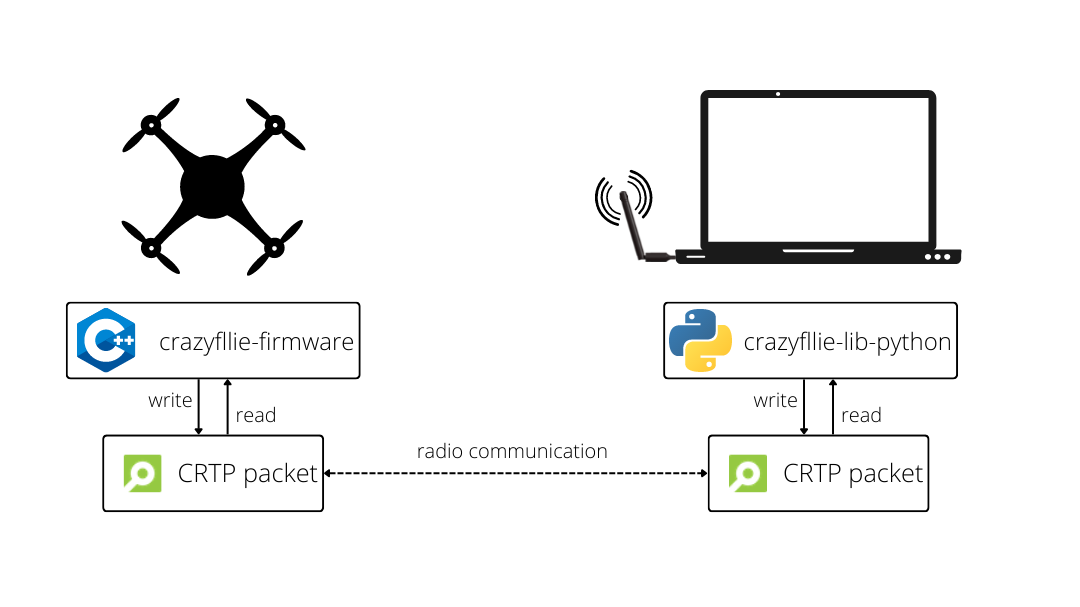
\includegraphics[width=0.9\textwidth]{tools/software_libraries}
    \caption[Software libraries integration]{
        The two main software libraries are \textit{crazyflie-firmware} and \textit{crazyflie-lib-python}. 
        The former, written in C++, runs on the drone; the latter, written in Python, runs on the base station. 
        The communication protocol that enables the cooperation of the two is the Crazy Radio Transfer Protocol (CRTP)}\label{fig:software_libraries}
\end{figure}


\section{Positioning Systems}\label{sec:positioning_systems}
Positioning systems represent the core sensing task of every drone application. 
Knowing the drone's position in the flight space is essential for achieving any possible goal.
We can identify two main categories of positioning systems: relative and absolute. 

Relative positioning systems are the simplest: starting from the drone's position at take-off, they estimate the position during the flight on the base of the movements made by the drone in the flight space. 
The measurement of the movements is usually made with the IMU (Inertial Measurement Unit) or with some additional sensors that track the difference in position over time.

The main issue related to this type of positioning system is that the error continually accumulates, and after a certain period of flight, they
can lead to consistent mispositioning~\cite{jametoni2021study}.

Absolute positioning systems provide coordinates that define the exact location of an object within a specific coordinate system. 
These systems typically rely on external references or signals from fixed anchors.
The sampling of the position in this type of positioning system is independent of any initial measurements, so the error in the positioning usually does not accumulate over time.


The Crazyflie platform offers multiple positioning systems, both absolute and relative. 
To select the best system for building our programming environment, we analyzed the following metrics for each possibility that the platform offered:
\begin{itemize}
    \item Accuracy in sampling
    \item Cumulative of the error during time
\end{itemize}


\subsection{Relative Positioning Systems}\label{subsec:relative_positioning_systems}
The Crazyflie platform offers three relative positioning systems. 
The first system is represented by the Inertial Measurement Unit, which is provided on the base drone without expansion decks. 
From our experience, this system has very poor accuracy and cannot be used as the only positioning system of the entire application.
However, it contributes its information to obtain the position estimate.

The Z-ranger deck (See~\ref{deck:z_ranger}) is another positioning system that the platform offers; it provides an estimate only for the z-coordinate with pretty good accuracy, but, as typical for every relative positioning system, it has a high cumulative error during the time. 

The Flow deck v2 (See~\ref{deck:flow}) represents an empowered version of the Z-ranger, a positioning system capable of measuring the distance from the takeoff point for the three coordinates x, y, and z. 
From our experiences, this last system has a good sampling accuracy and an acceptable cumulative error rate over time. 
Flow deck v2 is the only relative positioning system that allows the Crazyflie to fly with acceptable precision in the flight space.


\subsection{Absolute Positioning Systems}\label{subsec:absolute_positioning_systems}
The environment provides three different absolute positioning systems solutions with different characteristics, performance, and costs. 

The first solution proposed, the Loco Positioning System (LPS), is based on Ultra Wide Band radio that is used to find the absolute 3D position of objects in space. 
Similarly to a miniature GPS system, it uses a set of Anchors, namely Loco positioning nodes (from 4 up to 8), that act as a GPS satellite, and a Tag, 
namely, the Loco positioning deck, which acts as a GPS receiver. 
This system is highly subject to interference since it is based on radio signals that compute the position. 
The wi-fi signals and other radio-based technology make this system unusable inside the university's laboratories, where HDI researchers conduct their experiments.
In fact, as indicated in the specification of this system, the accuracy of this system is probably the main limitation and is estimated to be in the range of 10 cm. 

The second solution proposed is the Motion Capture System (MCS), which uses cameras to detect markers attached to the Crazyflies. 
Since the system knows the layout of the markers on the drone, it is possible to calculate the position and orientation of the tracked object in a global reference frame. 
It is a very accurate positioning system, but the two main limitations are that the native environment provides only the markers and relies on third-party systems for the entire MCS. 
Moreover, the position is computed in an external node and needs to be sent to the Crazyflie, increasing the communication load and latency.

The last solution is the Lighthouse positioning system (Lighthouse), the newest introduced in the environment and selected for the work because it overcomes some of the limitations of the other systems.
Lighthouse is an optically-based positioning system that allows an object to locate itself with high precision indoors. 

The system uses the SteamVR Base Station (BS) as an optical beacon. 
They are composed of spinning drums that shine the flight space with infrared beams in a range of 6 meters. 
The Crazyflie, on the other hand, with a Lighthouse positioning deck with four optical IR receivers (photodiode), can measure the angle of incidence of the IR beams. 
Knowing the position and orientation of the BS enables the Crazyflie to compute its position onboard in global coordinates. 
The knowledge of the position and the orientation of the BS is called system geometry and is composed of a vector in the three dimensions and a rotation matrix. 


\subsection{Lighthouse Positioning System Hardware}\label{subsec:lighthouse_hardware}
The Lighthouse positioning system is one of the possible solutions that Bitcraze offers to obtain an absolute positioning system for understanding the drone's coordinates inside the flight space. 
The hardware of this system is composed of 2 or more HTC-Vive/SteamVR Base Station 2.0. 
The role of these base stations is to lighten up the flight space with periodic infrared (IR) beams.

Onboard the Crazyflie 2.1, the Lighthouse expansion deck allows it to capture these IR beams thanks to four TS4231 IR receivers. 
The signal captured is then passed to an ICE40UP5K FPGA that computes the angle of incidence of the IR rays with signal processing. 
The position and the pose of the Craziflie are then finally computed from the main MCU of the Crazyflie 2.1
By precisely capturing and processing periodic infrared beams, the system enables Crazyflie 2.1 to determine its coordinates with accuracy and efficiency.

\section{State Estimate and Control}\label{sec:state_estimate_and_control}
All the information given by the positioning systems and by the additional decks are simply data,
to become useful, they need to be used cleverly to control the drone's stability and make it possible to fly. 

This section will describe the principal software components that act in the control loop, enabling the drone to fly.
In the Crazyflie platform, the control loop is managed inside the Crazyflie firmware (See~\ref{subsec:crazyflie-firmware}) from the sensor read to the motor thrust.
In Figure~\ref{fig:control_loop}, we can see a representation of the control loop of the Craziflie 2.1. 

\begin{figure}[tb]
    \centering
    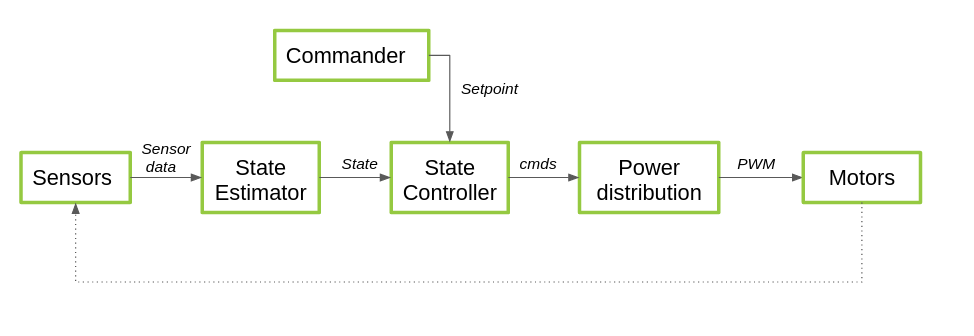
\includegraphics[width=0.9\textwidth]{tools/control_loop}
    \caption[Craziflie's control loop]{
        The control loop of the Craziflie 2.1~\cite{bitcraze}
    }\label{fig:control_loop}
\end{figure}

As in any feedback control system, also for the Crazyflie control loop, we can identify two principal components in Crazyflie 2.1: the state estimator and the state control. 
The synergy between the state estimate and the state control in a control loop is fundamental for achieving accurate and effective system control. 

The state estimator is responsible for computing the best possible estimate of the system's current status.
This component inside the Crazyflie 2.1 firmware has two concrete implementations with different performance and accuracy:
\begin{itemize}
    \item Complementary Filter
    \item Extended Kalman Filter (EKF)
\end{itemize}

The Complementary Filter is a very lightweight and efficient state estimator. 
It can only partially use the available sensors; in particular, it uses only data from the IMU and the ToF sensor (Flow deck or Z-ranger).
The estimated output is only a portion of the Crazyflie state: the Attitude (roll, pitch, and yaw) and the z coordinate relative to the starting point.

The EKF is a recursive filter that estimates the current state of the Crazyflie based on incoming measurements (in combination with a predicted standard deviation of the noise), the measurement model, and the model of the system itself. 
It is a step up in complexity with respect to the other estimator; it accepts all the possible sensors' data as input. 
If enough sensor data are available, it can compute a complete state estimation as output: Attitude, Position, and Velocity in all directions.
The choice of which state estimator to use can be forced by the user or automatically set. 
By default, the firmware uses the lighter Complementary Filter and switches to the EKF if more sensors are available.

The state control uses this estimate to elaborate the actions needed to change the current state to a target state.
On the Craziflie's 2.1 firmware, we have three possible alternatives, ordered by complexity:
\begin{itemize}
    \item Proportional Integral Derivative Controller (PID)
    \item Incremental Nonlinear Dynamic Inversion Controller (INDI)
    \item Mellinger Controller
\end{itemize}

The PID Controller offers simplicity and stability, making it suitable for straightforward applications. However, its effectiveness decreases in highly dynamic environments. 
INDI Controller excels in adapting to complex dynamics, but its sensitivity to parameter settings necessitates meticulous adjustments to maintain optimal performance.
Meanwhile, the Mellinger Controller prioritizes agility and responsiveness, making it well-suited for high-performance applications requiring quick and precise maneuvers. 


\section{Flight Control}\label{sec:flight_control}
On the other side of the communication channel, the ground station needs a way to interact with the drone and give information on which actions to take to fly in the desired way.


Inside the cflib the one responsible for controlling the flight is a module named Commander Framework.
The Commander Framework can be viewed as composed of two layers:

The first layer provides low-level operations that allow writing setpoints and sending them with the custom CRTP protocol.

The second layer, built upon the first, is more abstract and adds some general functionalities, e.g., take-off, land, and move-to.

To better understand the difference between these two levels of control, we will show the implementation of a simple example for both.


The scenario is the following:
\begin{displayquote}
    We must navigate the drone across four different waypoints for our developing drone application.
    In particular, starting from the takeoff position, we need to complete a squared trajectory passing through waypoints (1,0), (1,1), (0,1), and then back to (0,0).
\end{displayquote}

For the first implementation, using the low-level control mechanism (\textit{simple commander}), we have to consider that the Crazyflie needs a continuous flow of setpoints. 
In other words, each setpoint sent from the ground station is executed only for a limited period of 0.5 seconds.
The proposed solution must perform a timed loop to allow the Crazyflie to fly across the desired waypoints.
In addition, we also need to manually control the takeoff phase using the same timed loop technique.

In the Listing~\ref{example_simple_commander} is shown the resulting code for the simple implementation.

In the second implementation, using the more abstract layer (\textit{motion commander}), we can use the function \verb|move_distance| to perform the planned path.
In this example, the motion commander layer handles all the low-level issues and exposes a more simple and usable interface. 
Moreover, it automatically executes the takeoff and landing by specifying the default height.

The resulting script (Listing~\ref{example_motion_commander}) is more straightforward and readable.

\begin{figure}[tb]
    \centering
    \lstinputlisting[language=Python, caption={Waypoint navigation implemented using \textit{simple commander}}, label=example_simple_commander]{Scripts/tools_simple_commander.py}
\end{figure}
\begin{figure}[tb]
    \centering
    \lstinputlisting[language=Python, caption={Waypoint navigation implemented using \textit{motion commander}}, label=example_motion_commander]{Scripts/tools_motion_commander.py}
\end{figure}